% Options for packages loaded elsewhere
\PassOptionsToPackage{unicode}{hyperref}
\PassOptionsToPackage{hyphens}{url}
\PassOptionsToPackage{dvipsnames,svgnames,x11names}{xcolor}
%
\documentclass[
  letterpaper,
  DIV=11,
  numbers=noendperiod]{scrartcl}

\usepackage{amsmath,amssymb}
\usepackage{lmodern}
\usepackage{iftex}
\ifPDFTeX
  \usepackage[T1]{fontenc}
  \usepackage[utf8]{inputenc}
  \usepackage{textcomp} % provide euro and other symbols
\else % if luatex or xetex
  \usepackage{unicode-math}
  \defaultfontfeatures{Scale=MatchLowercase}
  \defaultfontfeatures[\rmfamily]{Ligatures=TeX,Scale=1}
\fi
% Use upquote if available, for straight quotes in verbatim environments
\IfFileExists{upquote.sty}{\usepackage{upquote}}{}
\IfFileExists{microtype.sty}{% use microtype if available
  \usepackage[]{microtype}
  \UseMicrotypeSet[protrusion]{basicmath} % disable protrusion for tt fonts
}{}
\makeatletter
\@ifundefined{KOMAClassName}{% if non-KOMA class
  \IfFileExists{parskip.sty}{%
    \usepackage{parskip}
  }{% else
    \setlength{\parindent}{0pt}
    \setlength{\parskip}{6pt plus 2pt minus 1pt}}
}{% if KOMA class
  \KOMAoptions{parskip=half}}
\makeatother
\usepackage{xcolor}
\setlength{\emergencystretch}{3em} % prevent overfull lines
\setcounter{secnumdepth}{-\maxdimen} % remove section numbering
% Make \paragraph and \subparagraph free-standing
\ifx\paragraph\undefined\else
  \let\oldparagraph\paragraph
  \renewcommand{\paragraph}[1]{\oldparagraph{#1}\mbox{}}
\fi
\ifx\subparagraph\undefined\else
  \let\oldsubparagraph\subparagraph
  \renewcommand{\subparagraph}[1]{\oldsubparagraph{#1}\mbox{}}
\fi

\usepackage{color}
\usepackage{fancyvrb}
\newcommand{\VerbBar}{|}
\newcommand{\VERB}{\Verb[commandchars=\\\{\}]}
\DefineVerbatimEnvironment{Highlighting}{Verbatim}{commandchars=\\\{\}}
% Add ',fontsize=\small' for more characters per line
\usepackage{framed}
\definecolor{shadecolor}{RGB}{241,243,245}
\newenvironment{Shaded}{\begin{snugshade}}{\end{snugshade}}
\newcommand{\AlertTok}[1]{\textcolor[rgb]{0.68,0.00,0.00}{#1}}
\newcommand{\AnnotationTok}[1]{\textcolor[rgb]{0.37,0.37,0.37}{#1}}
\newcommand{\AttributeTok}[1]{\textcolor[rgb]{0.40,0.45,0.13}{#1}}
\newcommand{\BaseNTok}[1]{\textcolor[rgb]{0.68,0.00,0.00}{#1}}
\newcommand{\BuiltInTok}[1]{\textcolor[rgb]{0.00,0.23,0.31}{#1}}
\newcommand{\CharTok}[1]{\textcolor[rgb]{0.13,0.47,0.30}{#1}}
\newcommand{\CommentTok}[1]{\textcolor[rgb]{0.37,0.37,0.37}{#1}}
\newcommand{\CommentVarTok}[1]{\textcolor[rgb]{0.37,0.37,0.37}{\textit{#1}}}
\newcommand{\ConstantTok}[1]{\textcolor[rgb]{0.56,0.35,0.01}{#1}}
\newcommand{\ControlFlowTok}[1]{\textcolor[rgb]{0.00,0.23,0.31}{#1}}
\newcommand{\DataTypeTok}[1]{\textcolor[rgb]{0.68,0.00,0.00}{#1}}
\newcommand{\DecValTok}[1]{\textcolor[rgb]{0.68,0.00,0.00}{#1}}
\newcommand{\DocumentationTok}[1]{\textcolor[rgb]{0.37,0.37,0.37}{\textit{#1}}}
\newcommand{\ErrorTok}[1]{\textcolor[rgb]{0.68,0.00,0.00}{#1}}
\newcommand{\ExtensionTok}[1]{\textcolor[rgb]{0.00,0.23,0.31}{#1}}
\newcommand{\FloatTok}[1]{\textcolor[rgb]{0.68,0.00,0.00}{#1}}
\newcommand{\FunctionTok}[1]{\textcolor[rgb]{0.28,0.35,0.67}{#1}}
\newcommand{\ImportTok}[1]{\textcolor[rgb]{0.00,0.46,0.62}{#1}}
\newcommand{\InformationTok}[1]{\textcolor[rgb]{0.37,0.37,0.37}{#1}}
\newcommand{\KeywordTok}[1]{\textcolor[rgb]{0.00,0.23,0.31}{#1}}
\newcommand{\NormalTok}[1]{\textcolor[rgb]{0.00,0.23,0.31}{#1}}
\newcommand{\OperatorTok}[1]{\textcolor[rgb]{0.37,0.37,0.37}{#1}}
\newcommand{\OtherTok}[1]{\textcolor[rgb]{0.00,0.23,0.31}{#1}}
\newcommand{\PreprocessorTok}[1]{\textcolor[rgb]{0.68,0.00,0.00}{#1}}
\newcommand{\RegionMarkerTok}[1]{\textcolor[rgb]{0.00,0.23,0.31}{#1}}
\newcommand{\SpecialCharTok}[1]{\textcolor[rgb]{0.37,0.37,0.37}{#1}}
\newcommand{\SpecialStringTok}[1]{\textcolor[rgb]{0.13,0.47,0.30}{#1}}
\newcommand{\StringTok}[1]{\textcolor[rgb]{0.13,0.47,0.30}{#1}}
\newcommand{\VariableTok}[1]{\textcolor[rgb]{0.07,0.07,0.07}{#1}}
\newcommand{\VerbatimStringTok}[1]{\textcolor[rgb]{0.13,0.47,0.30}{#1}}
\newcommand{\WarningTok}[1]{\textcolor[rgb]{0.37,0.37,0.37}{\textit{#1}}}

\providecommand{\tightlist}{%
  \setlength{\itemsep}{0pt}\setlength{\parskip}{0pt}}\usepackage{longtable,booktabs,array}
\usepackage{calc} % for calculating minipage widths
% Correct order of tables after \paragraph or \subparagraph
\usepackage{etoolbox}
\makeatletter
\patchcmd\longtable{\par}{\if@noskipsec\mbox{}\fi\par}{}{}
\makeatother
% Allow footnotes in longtable head/foot
\IfFileExists{footnotehyper.sty}{\usepackage{footnotehyper}}{\usepackage{footnote}}
\makesavenoteenv{longtable}
\usepackage{graphicx}
\makeatletter
\def\maxwidth{\ifdim\Gin@nat@width>\linewidth\linewidth\else\Gin@nat@width\fi}
\def\maxheight{\ifdim\Gin@nat@height>\textheight\textheight\else\Gin@nat@height\fi}
\makeatother
% Scale images if necessary, so that they will not overflow the page
% margins by default, and it is still possible to overwrite the defaults
% using explicit options in \includegraphics[width, height, ...]{}
\setkeys{Gin}{width=\maxwidth,height=\maxheight,keepaspectratio}
% Set default figure placement to htbp
\makeatletter
\def\fps@figure{htbp}
\makeatother
\newlength{\cslhangindent}
\setlength{\cslhangindent}{1.5em}
\newlength{\csllabelwidth}
\setlength{\csllabelwidth}{3em}
\newlength{\cslentryspacingunit} % times entry-spacing
\setlength{\cslentryspacingunit}{\parskip}
\newenvironment{CSLReferences}[2] % #1 hanging-ident, #2 entry spacing
 {% don't indent paragraphs
  \setlength{\parindent}{0pt}
  % turn on hanging indent if param 1 is 1
  \ifodd #1
  \let\oldpar\par
  \def\par{\hangindent=\cslhangindent\oldpar}
  \fi
  % set entry spacing
  \setlength{\parskip}{#2\cslentryspacingunit}
 }%
 {}
\usepackage{calc}
\newcommand{\CSLBlock}[1]{#1\hfill\break}
\newcommand{\CSLLeftMargin}[1]{\parbox[t]{\csllabelwidth}{#1}}
\newcommand{\CSLRightInline}[1]{\parbox[t]{\linewidth - \csllabelwidth}{#1}\break}
\newcommand{\CSLIndent}[1]{\hspace{\cslhangindent}#1}

\KOMAoption{captions}{tableheading}
\makeatletter
\makeatother
\makeatletter
\makeatother
\makeatletter
\@ifpackageloaded{caption}{}{\usepackage{caption}}
\AtBeginDocument{%
\ifdefined\contentsname
  \renewcommand*\contentsname{Table of contents}
\else
  \newcommand\contentsname{Table of contents}
\fi
\ifdefined\listfigurename
  \renewcommand*\listfigurename{List of Figures}
\else
  \newcommand\listfigurename{List of Figures}
\fi
\ifdefined\listtablename
  \renewcommand*\listtablename{List of Tables}
\else
  \newcommand\listtablename{List of Tables}
\fi
\ifdefined\figurename
  \renewcommand*\figurename{Figure}
\else
  \newcommand\figurename{Figure}
\fi
\ifdefined\tablename
  \renewcommand*\tablename{Table}
\else
  \newcommand\tablename{Table}
\fi
}
\@ifpackageloaded{float}{}{\usepackage{float}}
\floatstyle{ruled}
\@ifundefined{c@chapter}{\newfloat{codelisting}{h}{lop}}{\newfloat{codelisting}{h}{lop}[chapter]}
\floatname{codelisting}{Listing}
\newcommand*\listoflistings{\listof{codelisting}{List of Listings}}
\makeatother
\makeatletter
\@ifpackageloaded{caption}{}{\usepackage{caption}}
\@ifpackageloaded{subcaption}{}{\usepackage{subcaption}}
\makeatother
\makeatletter
\@ifpackageloaded{tcolorbox}{}{\usepackage[many]{tcolorbox}}
\makeatother
\makeatletter
\@ifundefined{shadecolor}{\definecolor{shadecolor}{rgb}{.97, .97, .97}}
\makeatother
\makeatletter
\makeatother
\ifLuaTeX
  \usepackage{selnolig}  % disable illegal ligatures
\fi
\IfFileExists{bookmark.sty}{\usepackage{bookmark}}{\usepackage{hyperref}}
\IfFileExists{xurl.sty}{\usepackage{xurl}}{} % add URL line breaks if available
\urlstyle{same} % disable monospaced font for URLs
\hypersetup{
  pdftitle={Salarios en Ciencia de Datos},
  pdfauthor={R-Ladies Medellín},
  colorlinks=true,
  linkcolor={blue},
  filecolor={Maroon},
  citecolor={Blue},
  urlcolor={Blue},
  pdfcreator={LaTeX via pandoc}}

\title{Salarios en Ciencia de Datos}
\author{R-Ladies Medellín}
\date{}

\begin{document}
\maketitle
\ifdefined\Shaded\renewenvironment{Shaded}{\begin{tcolorbox}[sharp corners, enhanced, boxrule=0pt, frame hidden, breakable, interior hidden, borderline west={3pt}{0pt}{shadecolor}]}{\end{tcolorbox}}\fi

\hypertarget{introduccion}{%
\subsection{Introduccion}\label{introduccion}}

En este análisis, cosntruimos un model que predice los salarios de los
profesionales basados en factores asociados a la persona y a la empresa.

\begin{Shaded}
\begin{Highlighting}[]
\FunctionTok{library}\NormalTok{(tidyverse)  }\CommentTok{\# Para la gestión y visualización de datos }
\end{Highlighting}
\end{Shaded}

\begin{verbatim}
Warning: package 'tidyverse' was built under R version 4.2.3
\end{verbatim}

\begin{verbatim}
Warning: package 'forcats' was built under R version 4.2.3
\end{verbatim}

\begin{verbatim}
Warning: package 'lubridate' was built under R version 4.2.3
\end{verbatim}

\begin{Shaded}
\begin{Highlighting}[]
\FunctionTok{library}\NormalTok{(knitr)      }\CommentTok{\# Para tablas}
\end{Highlighting}
\end{Shaded}

\begin{verbatim}
Warning: package 'knitr' was built under R version 4.2.3
\end{verbatim}

\begin{Shaded}
\begin{Highlighting}[]
\FunctionTok{library}\NormalTok{(broom)      }\CommentTok{\# Para el resumen del modelo}
\end{Highlighting}
\end{Shaded}

\begin{verbatim}
Warning: package 'broom' was built under R version 4.2.3
\end{verbatim}

\begin{Shaded}
\begin{Highlighting}[]
\FunctionTok{library}\NormalTok{(readr)      }\CommentTok{\# Para lectura de datos separados por csv}
\FunctionTok{library}\NormalTok{(ggplot2)}
\FunctionTok{library}\NormalTok{(hrbrthemes)}
\end{Highlighting}
\end{Shaded}

\begin{verbatim}
Warning: package 'hrbrthemes' was built under R version 4.2.3
\end{verbatim}

\begin{Shaded}
\begin{Highlighting}[]
\FunctionTok{library}\NormalTok{(scales)}

\NormalTok{salarios }\OtherTok{\textless{}{-}} \FunctionTok{read\_delim}\NormalTok{(}\StringTok{"ds\_salaries.csv"}\NormalTok{, }
    \AttributeTok{delim =} \StringTok{";"}\NormalTok{, }\AttributeTok{escape\_double =} \ConstantTok{FALSE}\NormalTok{, }
    \AttributeTok{col\_types =} \FunctionTok{cols}\NormalTok{(}\AttributeTok{work\_year =} \FunctionTok{col\_character}\NormalTok{(), }
                     \AttributeTok{remote\_ratio =} \FunctionTok{col\_character}\NormalTok{()))}
\end{Highlighting}
\end{Shaded}

Vamos a presentar los resultados del análisis de datos exploratorio en
Section~\ref{sec-aed} y el modelo de regresión en \textbf{?@sec-model}.

\hypertarget{sec-aed}{%
\subsection{Análisis exploratorio de datos}\label{sec-aed}}

Como parte del análisis de datos exploratorios vamos a visualizar la
relación entre el salario y el nivel de experiencia de los
profesionales.

\hypertarget{visualizaciuxf3n-de-datos}{%
\subsubsection{Visualización de datos}\label{visualizaciuxf3n-de-datos}}

Figure~\ref{fig-densbar} muestra la densidad de la distribución del
\texttt{salary\_in\_usd} y un diagrama de barras del
\texttt{experience\_level} de los profesionales.

\begin{Shaded}
\begin{Highlighting}[]
\FunctionTok{ggplot}\NormalTok{(salarios, }\FunctionTok{aes}\NormalTok{(}\AttributeTok{x =}\NormalTok{ salary\_in\_usd)) }\SpecialCharTok{+} 
  \FunctionTok{geom\_density}\NormalTok{(}\AttributeTok{fill=}\StringTok{"\#69b3a2"}\NormalTok{, }\AttributeTok{color=}\StringTok{"\#e9ecef"}\NormalTok{, }\AttributeTok{alpha=}\FloatTok{0.8}\NormalTok{) }\SpecialCharTok{+}
  \FunctionTok{labs}\NormalTok{(}\AttributeTok{y =} \StringTok{"Densidad"}\NormalTok{) }\SpecialCharTok{+} 
  \FunctionTok{scale\_x\_continuous}\NormalTok{(}\AttributeTok{labels  =} \FunctionTok{label\_number}\NormalTok{(}\AttributeTok{scale =} \FloatTok{1e{-}3}\NormalTok{, }\AttributeTok{prefix =} \StringTok{"$"}\NormalTok{, }
                                            \AttributeTok{suffix =} \StringTok{"m"}\NormalTok{, }\AttributeTok{accuracy =} \DecValTok{1}\NormalTok{)) }

\FunctionTok{ggplot}\NormalTok{(salarios, }\FunctionTok{aes}\NormalTok{(}\AttributeTok{x =}\NormalTok{ experience\_level, }\AttributeTok{fill =}\NormalTok{ experience\_level)) }\SpecialCharTok{+} 
  \FunctionTok{geom\_bar}\NormalTok{() }\SpecialCharTok{+}
  \FunctionTok{scale\_fill\_brewer}\NormalTok{(}\AttributeTok{palette=}\StringTok{"GnBu"}\NormalTok{)  }\SpecialCharTok{+} 
  \FunctionTok{labs}\NormalTok{(}\AttributeTok{x =} \StringTok{"Nivel de experiencia"}\NormalTok{, }\AttributeTok{y =} \StringTok{"Número de empleados analizados"}\NormalTok{)}
\end{Highlighting}
\end{Shaded}

\begin{figure}

\begin{minipage}[t]{0.50\linewidth}

{\centering 

\raisebox{-\height}{

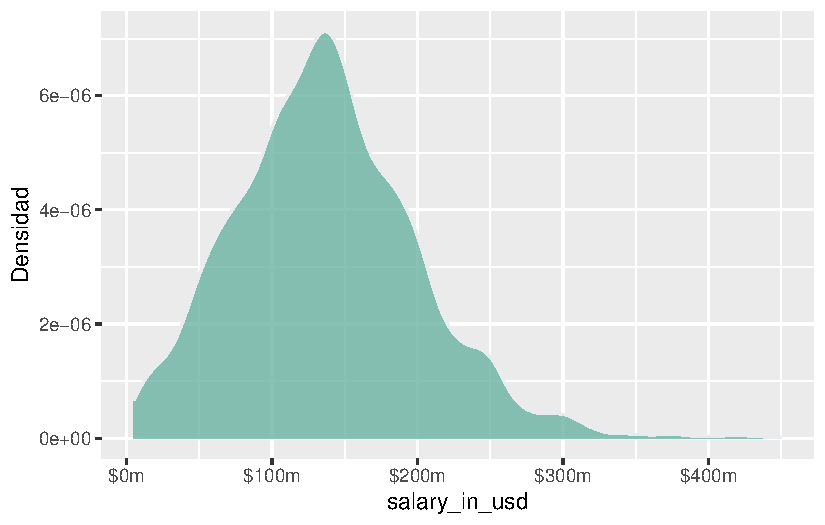
\includegraphics{Autoría_files/figure-pdf/fig-densbar-1.pdf}

}

}

\subcaption{\label{fig-densbar-1}Densidad de \texttt{salary\_in\_usd}}
\end{minipage}%
%
\begin{minipage}[t]{0.50\linewidth}

{\centering 

\raisebox{-\height}{

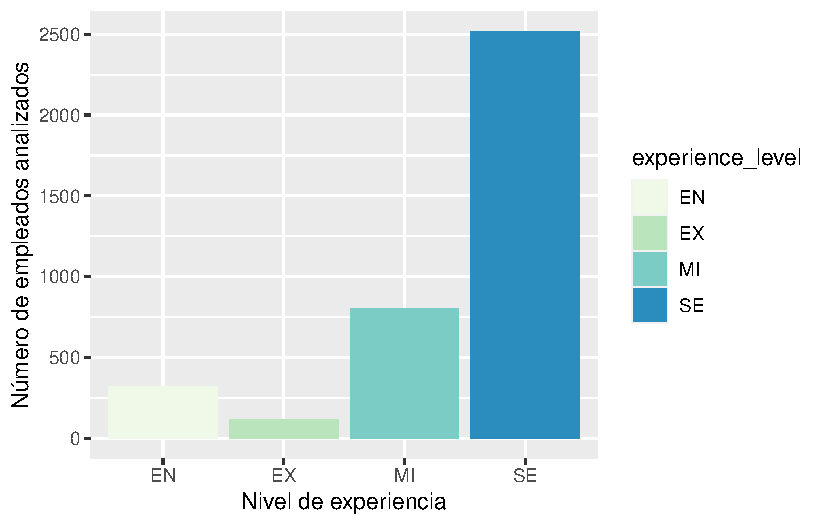
\includegraphics{Autoría_files/figure-pdf/fig-densbar-2.pdf}

}

}

\subcaption{\label{fig-densbar-2}Diagrama de barras de
\texttt{experience\_level}}
\end{minipage}%

\caption{\label{fig-densbar}Densidad y diagrama de barras de salario y
nivel de experiencia}

\end{figure}

Figure~\ref{fig-boxplotcomp} dmuestra la relación entre salarios y nivel
de experiencia de profesionales.

\begin{Shaded}
\begin{Highlighting}[]
\FunctionTok{ggplot}\NormalTok{(salarios, }\FunctionTok{aes}\NormalTok{(}\AttributeTok{x=}\NormalTok{salary\_in\_usd, }\AttributeTok{group=}\NormalTok{experience\_level, }\AttributeTok{fill=}\NormalTok{experience\_level, }\AttributeTok{col =}\NormalTok{ experience\_level)) }\SpecialCharTok{+}
  \FunctionTok{geom\_density}\NormalTok{(}\AttributeTok{adjust=}\FloatTok{1.5}\NormalTok{, }\AttributeTok{alpha=}\NormalTok{.}\DecValTok{6}\NormalTok{) }
  \FunctionTok{ylab}\NormalTok{(}\StringTok{""}\NormalTok{) }
\end{Highlighting}
\end{Shaded}

\begin{verbatim}
$y
[1] ""

attr(,"class")
[1] "labels"
\end{verbatim}

\begin{figure}[H]

{\centering 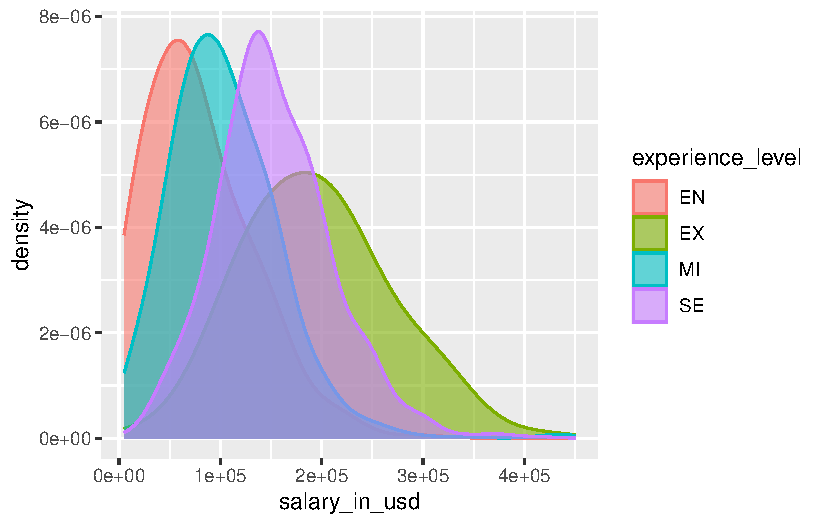
\includegraphics{Autoría_files/figure-pdf/fig-boxplotcomp-1.pdf}

}

\caption{\label{fig-boxplotcomp}Salario vs Nivel de experiencia}

\end{figure}

\hypertarget{summary-statistics}{%
\subsubsection{Summary statistics}\label{summary-statistics}}

Table~\ref{tbl-stats} muestra resumen estadístico para estas dos
variables.

\begin{Shaded}
\begin{Highlighting}[]
\NormalTok{salarios }\SpecialCharTok{\%\textgreater{}\%}
  \FunctionTok{summarise}\NormalTok{(}
    \StringTok{\textasciigrave{}}\AttributeTok{Mediana de Salario}\StringTok{\textasciigrave{}} \OtherTok{=} \FunctionTok{median}\NormalTok{(salary\_in\_usd),}
    \StringTok{\textasciigrave{}}\AttributeTok{RIC salario}\StringTok{\textasciigrave{}} \OtherTok{=} \FunctionTok{IQR}\NormalTok{(salary\_in\_usd)}
\NormalTok{  ) }\SpecialCharTok{\%\textgreater{}\%}
  \FunctionTok{kable}\NormalTok{(}\AttributeTok{digits =} \FunctionTok{c}\NormalTok{(}\DecValTok{0}\NormalTok{, }\DecValTok{0}\NormalTok{))}
\end{Highlighting}
\end{Shaded}

\hypertarget{tbl-stats}{}
\begin{longtable}[]{@{}rr@{}}
\caption{\label{tbl-stats}Resumen estadístico de salarios vs Nivel de
experiencia}\tabularnewline
\toprule()
Mediana de Salario & RIC salario \\
\midrule()
\endfirsthead
\toprule()
Mediana de Salario & RIC salario \\
\midrule()
\endhead
135000 & 80000 \\
\bottomrule()
\end{longtable}

\hypertarget{sec-modelo}{%
\subsection{Modelación}\label{sec-modelo}}

Ajustamos un modelo de regresión lineal simple de la forma mostrada en
la ecuación Equation~\ref{eq-modelo}.

\begin{equation}\protect\hypertarget{eq-modelo}{}{
Salario = \hat{\beta}_0 + \hat{\beta}_1 \times Experiencia + \epsilon
}\label{eq-modelo}\end{equation}

Table~\ref{tbl-lm} muestra la salida del modelo de regresión.

\begin{Shaded}
\begin{Highlighting}[]
\NormalTok{salario\_modelo }\OtherTok{\textless{}{-}} \FunctionTok{lm}\NormalTok{(salary\_in\_usd }\SpecialCharTok{\textasciitilde{}}\NormalTok{ experience\_level, }\AttributeTok{data =}\NormalTok{ salarios)}

\NormalTok{salario\_modelo }\SpecialCharTok{\%\textgreater{}\%}
  \FunctionTok{tidy}\NormalTok{() }\SpecialCharTok{\%\textgreater{}\%}
  \FunctionTok{kable}\NormalTok{(}\AttributeTok{digits =} \FunctionTok{c}\NormalTok{(}\DecValTok{0}\NormalTok{, }\DecValTok{0}\NormalTok{, }\DecValTok{2}\NormalTok{, }\DecValTok{2}\NormalTok{, }\DecValTok{2}\NormalTok{))}
\end{Highlighting}
\end{Shaded}

\hypertarget{tbl-lm}{}
\begin{longtable}[]{@{}lrrrr@{}}
\caption{\label{tbl-lm}Modelo de regresión lineal de salarios vs nivel
de experiencia}\tabularnewline
\toprule()
term & estimate & std.error & statistic & p.value \\
\midrule()
\endfirsthead
\toprule()
term & estimate & std.error & statistic & p.value \\
\midrule()
\endhead
(Intercept) & 78546 & 3155.80 & 24.89 & 0 \\
experience\_levelEX & 116385 & 6157.46 & 18.90 & 0 \\
experience\_levelMI & 25980 & 3730.68 & 6.96 & 0 \\
experience\_levelSE & 74505 & 3350.48 & 22.24 & 0 \\
\bottomrule()
\end{longtable}

El articulo (Das, Barik, and Mukherjee 2020) presenta un análisis de la
predicción del salario usando métodos de regresión.

\hypertarget{referencias}{%
\subsection*{Referencias}\label{referencias}}
\addcontentsline{toc}{subsection}{Referencias}

\hypertarget{refs}{}
\begin{CSLReferences}{1}{0}
\leavevmode\vadjust pre{\hypertarget{ref-das2020}{}}%
Das, Sayan, Rupashri Barik, and Ayush Mukherjee. 2020. {``Salary
Prediction Using Regression Techniques.''} \emph{SSRN Electronic
Journal}. \url{https://doi.org/10.2139/ssrn.3526707}.

\end{CSLReferences}



\end{document}
